\documentclass[11pt]{article}

%\usepackage[english]{babel}
\usepackage[utf8]{inputenc} %German Umlaute :-)
%\usepackage{apacite} %won't work for Greg, will work for Eva
\usepackage{natbib} %will work for Greg & Judith, won't work for Eva
\usepackage{amsmath,amssymb}
\usepackage{graphicx}
\usepackage{color}
\usepackage{url}
\usepackage{fullpage}
\usepackage{setspace}
\usepackage{booktabs}
%\usepackage{lingmacros}
\usepackage{gb4e}
\usepackage{hyperref}
\hypersetup{colorlinks,breaklinks,
            linkcolor=cyan,urlcolor=cyan,
            anchorcolor=cyan,citecolor=cyan}


% useful commands
\definecolor{Red}{RGB}{255,0,0}
\newcommand{\red}[1]{\textcolor{Red}{#1}}
\newcommand{\jd}[1]{\textcolor{Red}{[jd: #1]}} 

\newcommand{\denote}[1]{\mbox{ $[\![ #1 ]\!]$}}
\newcommand{\subsubsubsection}[1]{{\em #1}}
\newcommand{\eref}[1]{(\ref{#1})}
\newcommand{\tableref}[1]{Table \ref{#1}}
\newcommand{\figref}[1]{Figure \ref{#1}}
\newcommand{\appref}[1]{Appendix \ref{#1}}
\newcommand{\sectionref}[1]{Section \ref{#1}}


%for margin notes
\usepackage{marginnote, setspace}
\newcommand{\evanote}[1]{%
   \marginnote{%
      \begin{spacing}{1}
         \vspace{-\baselineskip}%
         \color{OliveGreen}\footnotesize\singlespacing\itshape#1
      \end{spacing}
   }
}

\newcommand{\gcs}[1]{\textcolor{blue}{[gcs: #1]}} 

\title{Definitely, maybe: Approaching speaker commitment experimentally}
 
\author{{\large \bf Judith Degen (jdegen@stanford.edu)}, \\ {\large \bf Andreas Trotzke (trotzke@stanford.edu),}\\ {\large \bf Gregory Scontras (scontras@stanford.edu),}\\  {\large \bf Eva Wittenberg (ewittenberg@ucsd.edu)}\\ {\large \bf Noah D.~Goodman (ngoodman@stanford.edu)}}



\begin{document}

\maketitle

\begin{abstract}

We present a series of experiments investigating the interaction between speakers’ choice of closely-related evidential expressions and the respective strength of speaker commitment that is conveyed. Specifically, we examine the extent to which listeners' interpretation of certain types of modals and their judgments about speaker commitment differ in strength, comparing the epistemic use of \emph{must} to the use of discourse particles, and to statements with no evidential markers. We also probe speakers' production preferences for these different devices under varying evidential circumstances. The results of our experiments confirm differences already observed in the literature. In addition, our data shed some new light on traditional assumptions. In particular, they challenge prominent accounts treating epistemic \emph{must} and other modals in parallel by encoding the epistemic reading into the lexical semantics of \emph{must}. We show that \emph{must} both differs from other modals and parallels use-conditional devices such as discourse particles. We conclude that our experimental squib provides a good starting point for approaching theoretical debates on the nature of evidential expressions empirically.

\end{abstract}

\textbf{Keywords:} 
evidentials; modals; discourse particles; English; German; pragmatics; psycholinguistics


\section{Introduction}

When speakers are certain about some fact expressed by a proposition \emph{p} (e.g., that the coffee is cold), they are likely to communicate this fact with a simple declarative utterance, as in (\ref{bare}). When they want to convey epistemic uncertainty, they have different devices for doing so: adding a modal adverbial, such as \emph{probably} (\ref{prob}), or using a modal verb, such as \emph{might} (\ref{might}). Either option leaves open the possibility that \emph{p} is not true.

\begin{exe}
	\ex\label{english} \begin{xlist}
		\ex\label{bare} The coffee is cold.
		\ex\label{prob} The coffee is probably cold.
		\ex\label{might} The coffee might be cold.
		\ex\label{must} The coffee must be cold.
	\end{xlist}
\end{exe}


While it is uncontroversial that in both (\ref{prob}) and (\ref{might}) epistemic uncertainty is conveyed by lexical means, it is a hotly debated issue whether the uncertainty communicated by (\ref{must}) reduces to the same interpretive mechanism. Note that the relative weakness of \emph{must} (i.e., it yields a weaker claim than (\ref{bare}), cf. \citealp{karttunen1972}) is puzzling because \emph{must} serves as a strong modal of necessity. Under a quantificational treatment of modality, such necessity modals correspond to universal quantifiers over possible worlds (e.g., \citealp{kratzer1991}). They assert that in every (relevant) possible world, the proposition \emph{p} holds. So in (\ref{must}), epistemic \emph{must} should assert that in every world compatible with the speaker's knowledge, the coffee is cold. Given that knowledge corresponds to justified true belief (i.e., that which is known cannot be otherwise), from (\ref{must}) it necessarily follows that the coffee is cold (i.e., it is not possible that the coffee is not cold).

At issue, then, is the failed inference from (\ref{must}) to (\ref{bare}): how could \emph{must p} not entail \emph{p}? If the coffee is necessarily cold, then surely it is cold. However, it appears that talking about what is \emph{necessarily} the case commits speakers to less than does talking about what is \emph{actually} the case. We could pose the question instead from a comprehension perspective: How do listeners understand that \emph{p} does not necessarily follow from \emph{must p}? Given this puzzle, one could hypothesize that the weakness of epistemic \emph{must} need not derive from truth-conditional content (e.g., quantification over a limited set of possible worlds or presuppositions about evidence strength). Rather, the epistemic interpretation of \emph{must} may rely on contextual factors such as evidence strength and thus may involve active pragmatic reasoning on the part of the listener.

Other languages have many more ways to convey weakened speaker commitment (for an overview, see \citealp{Aikhenvald2004,Drubig2001,Nuyts2001}). Even within the group of Germanic languages, we observe striking differences. German, for instance, is an interesting comparison case to English. While many devices for expressing speaker certainty do not differ from English (examples \ref{bareG}-\ref{mustG} are the German equivalents to \ref{bare}, \ref{prob}, and \ref{must}), German possesses a class of so-called `discourse particles' to which English is not privy: (\ref{wohlG}) is an example involving the discourse particle \emph{wohl} \citep{Zimmermann2004}. 

\begin{exe}
	\ex\label{german} \begin{xlist}
		\ex\label{bareG} \gll Der Kaffee ist kalt geworden. \\
		The coffee has cold become\\
		\glt `The coffee has become cold.'
				
		\ex\label{probG} \gll Der Kaffee ist vermutlich kalt geworden.\\
				The coffee has presumably cold become\\
		\glt `The coffee has presumably become cold.'

		\ex\label{mustG} \gll Der Kaffee muss kalt geworden sein. \\
						The coffee must  cold become have\\
		\glt `The coffee must have become cold.'
		\ex\label{wohlG} \gll Der Kaffee ist wohl kalt geworden.\\
						The coffee has PRT cold become\\
		\glt lit.: `The coffee has presumably become cold.'
	\end{xlist}
\end{exe}

Discourse particles like \emph{wohl} organize the discourse by conveying the epistemic states of both the speaker and the hearer. What is interesting about (\ref{wohlG}) for our purposes is that discourse particles such as \emph{wohl}, although lexically encoding weakened speaker commitment, are not part of the propositional, truth-conditional content of an utterance, in contrast to modal adverbs such as \emph{vermutlich} (`presumably’) in (\ref{probG}). Consider the following examples by \citet[][p.~2013]{Zimmermann2011}:

\begin{exe}
\ex \label{dparticles}
\begin{xlist}
\ex \gll Max ist	ja auf See.\\
Max is	 PRT at sea\\
\trans `(As I and you assume) Max is at sea.'
\ex \gll Max ist doch auf See.\\
Max is	 PRT at sea\\
\trans `(As you should know) Max is at sea.'
\ex \gll Max ist wohl auf See.\\
Max is	PRT at	sea\\
\trans `(As you may know) Max is at sea.'
\end{xlist}
\end{exe}

Roughly, \emph{ja} conveys that both the speaker and the hearer may already know the proposition, \emph{doch} expresses that the hearer should update his knowledge concerning the proposition, and \emph{wohl} articulates that the speaker merely assumes that the propositional content is true. Discourse particles are optional; leaving them out does not affect the truth conditions of a sentence: All the variants in (\ref{dparticles}) are true if Max is at sea, regardless of what kind of speaker commitment is conveyed by the discourse particles.

%\begin{exe}
%\ex \gll Max ist auf See { , ja, doch, wohl}\\
%Max is at sea PRT\\
%\trans `Max is at sea.' \gcs{check translation}
%\end{exe}

As with the epistemic use of \emph{must} (\ref{must})/(\ref{mustG}), \emph{wohl} is thus a special case of expressing weakened speaker commitment. Specifically, \cite{Zimmermann2004, Zimmermann2008} has shown that this particular particle cannot affect the presuppositional domain of utterance interpretation, unlike modal adverbs such as \emph{vermutlich} `presumably'. If \emph{wohl} contributed to the proposition semantically, its use in the following case should have the effect that the focus presupposition is an assumption rather than an actual state of affairs (capitals indicate focal stress):

\begin{exe}
\ex \label{wohl}
\begin{xlist}
\ex \gll Peter	ist	\{ \#	wohl  /	vermutlich\}	GESTERN			nach	 Hamburg	 gefahren	\\
		Peter	is		\{ \#	PRT  /   presumably\}	yesterday 		to	 Hamburg	 driven	\\	
\glt `Peter \{PRT/presumably\} went to Hamburg yesterday.'
\ex \label{wohlb} \gll \ldots vielleicht fährt er aber	auch erst MORGEN\\
\ldots maybe drives he but also only tomorrow\\
\glt `\ldots but maybe he will only go tomorrow.' 
\end{xlist}
\end{exe}
	
	
However, (\ref{wohl}) indicates that only the modal adverb \emph{vermutlich} can be mapped onto the focus presupposition that Peter went to Hamburg YESTERDAY. In other words, \emph{vermutlich} turns the focus presupposition into an assumption. It thus follows that only the modal adverb, and not the discourse particle, is felicitous given the continuation in (\ref{wohlb}), which expresses an assertion that is in conflict with the presupposition of the utterance without \emph{wohl} or \emph{vermutlich}. Based on such evidence, many researchers have argued that discourse particles like \emph{wohl}, although in principle synonymous with certain adverbs (here: \emph{vermutlich}), operate within a separate, `use-conditional' dimension of meaning (cf. \citealp[][pp.~215--268]{Gutzmann2015}, for more arguments).

This cross-linguistic sketch of expressions conveying different strengths of speaker commitment is based on subtle judgments of sentences containing modals and discourse particles, and there is to date very little empirical work that attempts to systematically evaluate different aspects of the use of evidential devices (though cf. \citealp{KnobeYalcin2014}; \citeauthor{LassiterInpress}, in press). We intend the experiments reported here to provide a more articulated road map for such an empirical investigation. In particular, we address the following questions: (i) Under which evidential circumstances do speakers prefer to use which evidential devices?  Put differently, how do speakers use the various evidential devices? and (ii) Do listeners ascribe different strengths of speaker commitment to the use of these various linguistic devices? In other words, how do listeners interpret speakers' use of these devices? Before directly addressing these questions, we first introduce our experimental materials and obtain estimates of evidence strength. These data will then serve as the basis for the analyses that follow.

\section{Experiment 1: evidence strength}

To investigate the role of evidence strength in the production and comprehension of evidential devices, we must first generate a set of pieces of evidence that vary in how strongly they provide support for a proposition $p$. To that end, Exp.~1 collected estimates of evidence strength.\footnote{The English version of this experiment can be viewed \href{https://web.stanford.edu/~justinek/modals_exp/evidence.html}{here}. The German version can be viewed \href{http://web.stanford.edu/~jdegen/cgi-bin/4_dp_priors_evidencestrength/evidence.html}{here}.} These estimates were used in the analyses of Experiments 2 and 3.

\subsection{Methods}

\subsubsection{Participants}

For the English version, 40 native English speakers were recruited through Amazon's Mechanical Turk crowd-sourcing service. For the German version, 40 German native speakers were recruited through Clickworker's crowd-sourcing service. Both groups were compensated for their participation.

\subsubsection{Materials and procedure}

Participants rated the probability of a state of affairs $p$ given a piece of evidence $e$ by adjusting a slider on a scale with endpoints labeled ``impossible'' and ``absolutely certain.''\footnote{Pieces of evidence were generated through a separate free production paradigm.  A speaker's description of some state of affairs $p$ was given to participants and they were asked to provide a free response explanation of how the speaker knew about $p$. This experiment can be viewed \href{http://stanford.edu/~jdegen/68_modals_freeproduction/modals.html}{here}. Similar responses (e.g., ``he can hear it'' and ``he can hear it on the roof'') were grouped together. We selected explanations from among the most frequently generated ones while including at least one of each type of evidence (direct, indirect, reportative) in the final selection of five pieces of evidence per domain. All materials were translated into German by authors 1, 2, and 4, who are native speakers of German.} On each trial, participants first saw the following context sentence: ``Imagine that you are at home.'' Then the evidence $e$ for $p$ was shown, e.g., ``Dinner is usually ready around 6pm. You look at the clock and it is 6pm.'' Finally, participants were asked about the probability of $p$, e.g., ``How likely is it that dinner is ready?'' and adjusted the slider accordingly. There were four different states of affairs $p$ that appeared in the ``How likely is it that $p$?'' frame:

\begin{exe}
\ex
\begin{xlist}
	\ex it is raining
	\ex the coffee is cold
	\ex dinner is ready
	\ex the neighbor's dog is barking
	\end{xlist}
\end{exe}

For each \emph{p}, each participant evaluated one of five possible pieces of evidence, resulting in four trials per participant. Trial order was randomized. 
For the German version, the procedure was identical; all materials were translated into German. See \appref{sec:evidence} for the full list of stimuli.

\subsection{Results and discussion}

We obtained between 3 and 14 strength ratings for each piece of evidence. We interpret the slider value between 0 (``impossible'') and 1 (``absolutely certain'') as a participant's estimate of the probability of $p$ given $e$, which we will also refer to as  \emph{evidence strength}. Strength of each piece of evidence in both the English and German task is shown in \figref{fig:evidencestrength}.  We used these pieces of evidence in the design of Experiments 2 and 3; analyses employed evidence strength means (indicated by black dots in the Figure).

\begin{figure}
\centering
%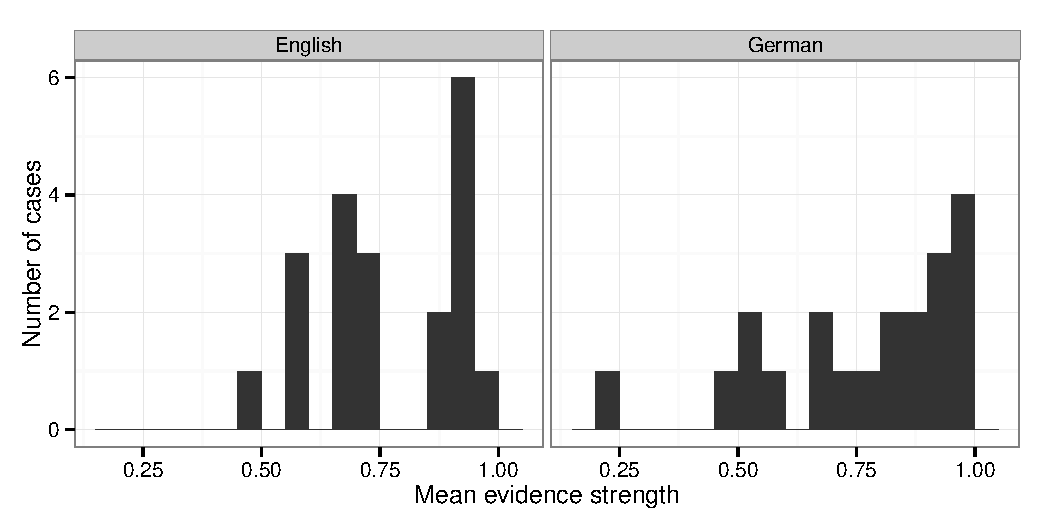
\includegraphics[width=.9\textwidth]{pics/evidencestrength-histograms}
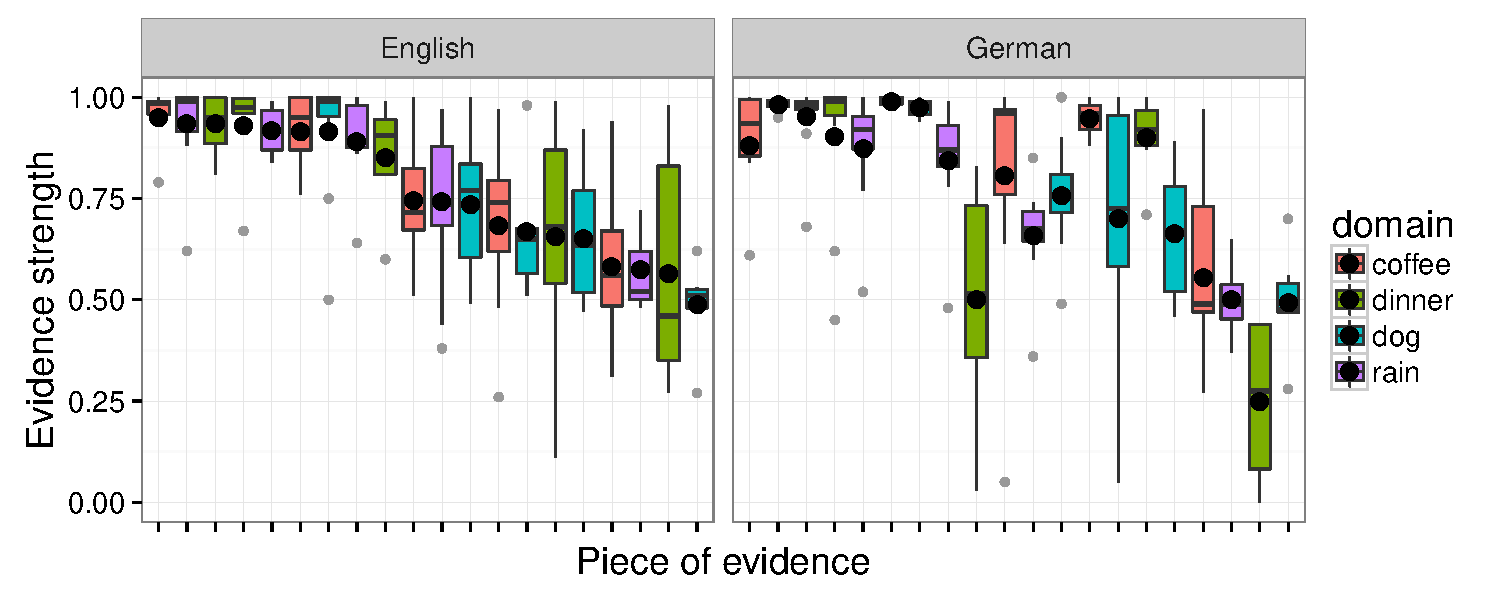
\includegraphics[width=\textwidth]{pics/evidencestrength-boxplots}
\caption{Boxplots of by-item evidence strength  for English (left) and German (right). Pieces of evidence occur in same order in English and German panel and are sorted by the English means. Horizontal lines indicate medians, black dots indicate means. Boxes indicate the range into which 50\% of the data fall. Whiskers extend to 1.5 times the interquartile range.}
\label{fig:evidencestrength}
\end{figure}


To test whether the English and German distributions of strength ratings differed, we conducted a mixed-effects linear regression predicting evidence strength rating from a dummy-coded fixed effect of language (with English as reference level) as well as by-participant and by-item random intercepts and by-item random slopes for language. The effect of language did not reach significance ($\beta$ = -.01, $SE$ = .03, $t$ = -.22, $p <$ .83), suggesting that the two populations did not differ in their estimates of evidence strength.   

\section{Experiment 2: production}


Ex.~2 addressed the first main question of interest: under what evidential circumstances do speakers use which evidential devices? In other words, what are the evidential use conditions for the various cross-linguistic devices we focus on? We thus investigate the interaction between speakers’ choice of closely-related evidential expressions and concrete scenarios.  To this end, we evaluated speakers' intuitions in a forced production task, testing how likely they are to use a particular evidential device to communicate their belief about $p$ when confronted with pieces of evidence that differ in how strongly they support $p$.\footnote{The English version of this experiment can be viewed \href{http://stanford.edu/~jdegen/71_modals_forced_production/modals.html}{here}.} The German version was identical with the exception that it was conducted in German and contained slightly different utterance choices (explained below).\footnote{The German version of this experiment can be viewed \href{http://web.stanford.edu/~jdegen/cgi-bin/3_dp_production/modals.html}{here}.}

\subsection{Methods}

\subsubsection{Participants}

For the English version, we recruited 40 participants from Amazon's Mechanical Turk. For the German version, we recruited 40 participants on the German crowd-sourcing service Clickworker. Participants were compensated for their participation.

\subsubsection{Materials and procedure}

Participants were asked to choose one of four possible utterances to describe the situation to a friend. On each trial, they first saw a context sentence which varied by domain, e.g., ``Imagine that you are sitting in a room.'' Next, they were presented with a piece of evidence, e.g., ``Earlier today, you saw dark clouds in the sky.'' Finally, each participant saw the same question: ``Given what you know, what do you say to a friend who is sitting in a windowless room down the hall?'' They then chose one of four possible utterances by checking a radio button, e.g., ``It's raining,’’ ``It must be raining,’’ ``It's probably raining,’’ ``It might be raining.’’ Depending on the language of testing, possible utterances took the forms shown in \eref{utterancechoices} or \eref{gutterancechoices}; for German we included the bare $p$ form and \emph{must p} as in the English version, but instead of the modals \emph{probably} and \emph{might}, we included the modal adverbial \emph{vermutlich} (English \emph{presumably}) and the discourse particle \emph{wohl}. This will allow us to compare not only certain types of modals to the epistemic use of \emph{must} (and to statements with no evidential markers at all), but also to compare both modals and \emph{must} to exceptional means such as discourse particles. 


\begin{exe}
	\ex\label{utterancechoices} \emph{Abstract form of English utterance choices:}
	\begin{xlist}
		\ex $p$ (bare)
		\ex \emph{must p} (must)
		\ex \emph{probably p} (probably)
		\ex \emph{might p} (might)
		\end{xlist}
	\ex\label{gutterancechoices} \emph{Abstract form of German utterance choices:}
	\begin{xlist}
		\ex $p$ (bare)
		\ex \emph{muss p} (muss)
		\ex \emph{wohl p} (wohl)
		\ex \emph{vermutlich p} (vermutlich)
		\end{xlist}
		\end{exe}
		
Each participant completed 12 trials, three per domain. For each participant and domain, three pieces of evidence were randomly sampled from the set of five. Trial order was randomized, as was the order of utterance options.

%The procedure for German was identical. As for participants' utterance choices, w

\subsection{Results and discussion}

The overall distribution of utterance choices is shown in \figref{fig:utterances}. In both English and German, the bare form is used most frequently. In English, \emph{might} is also used frequently, with both \emph{must} and \emph{probably} being chosen at only half the rate. A similar picture obtains in German, where \emph{muss p} is generally dispreferred.

The main question of interest  is whether the choice of form to communicate about $p$ depends on the strength of the evidence for $p$. Indeed, it does: \figref{fig:utterances-estrength} shows the mean strength of the evidence (as elicited in Exp.~1) that participants were given as a function of the utterance they ultimately chose. \figref{fig:utterances-by-strength} shows the proportion with which each utterance was chosen as a function of evidence strength.   In order to evaluate the effect of evidence strength on utterance choice, we conducted two separate mixed-effects linear regressions -- one for the English data, one for the German data -- predicting evidence strength from a dummy-coded predictor for utterance choice. In both cases, \emph{must}/\emph{muss} served as reference level. The models included random by-participant and by-item  intercepts. Evidence strength was greater when the bare form was produced than when \emph{must/muss q} was produced in both English ($\beta$ = .11, $SE$ = .01, $t$ = 7.58, $p <$ .0001) and German ($\beta$ = .12, $SE$ = .03, $t$ = 4.78, $p <$ .0001). In English, evidence   was weaker  when \emph{might p} was produced  ($\beta$ = -.13, $SE$ = .01, $t$ = -8.99, $p <$ .0001). There was no difference in evidence strength between \emph{must p} and \emph{probably p}  ($\beta$ = -.01, $SE$ = .02, $t$ = -.73, $p <$ .47). In German, evidence was weaker when \emph{vermutlich p} was produced  ($\beta$ = -.09, $SE$ = .03, $t$ = -3.35, $p <$ .0009). Interestingly, there was no difference in evidence strength between \emph{muss p} and \emph{wohl p}  ($\beta$ = -.02, $SE$ = .03, $t$ = -.67, $p <$ .51).

\begin{figure}
\centering
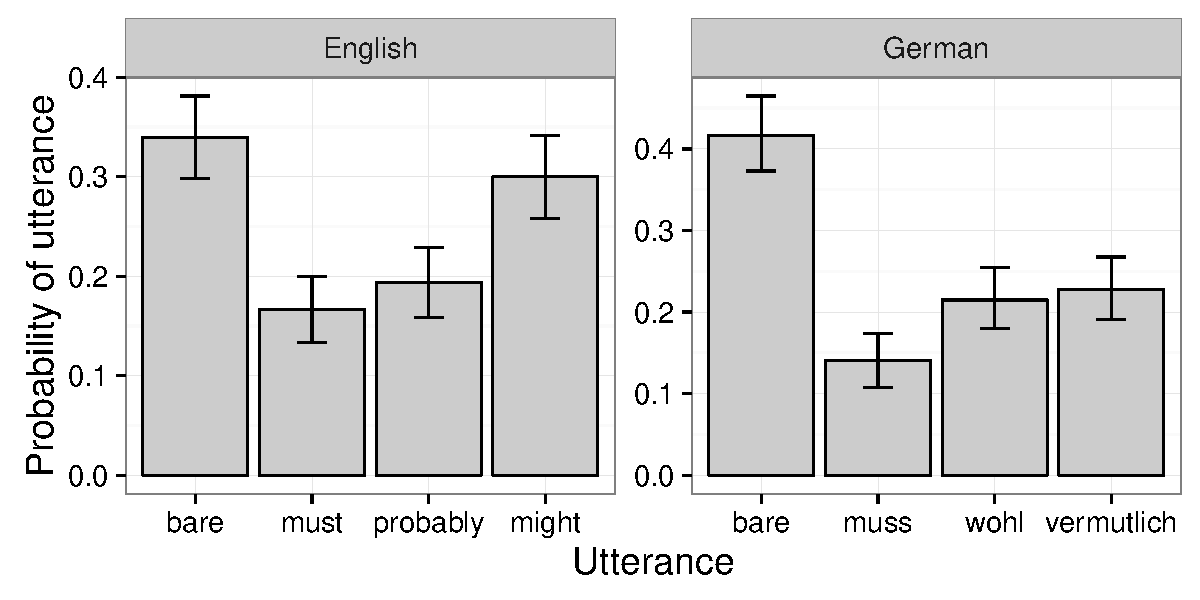
\includegraphics[width=.9\textwidth]{pics/production-distribution}
\caption{Probability of utterance choice for English (left) and German (right). Error bars indicate bootstrapped 95\% confidence intervals.}
\label{fig:utterances}
\end{figure}



\begin{figure}
\centering
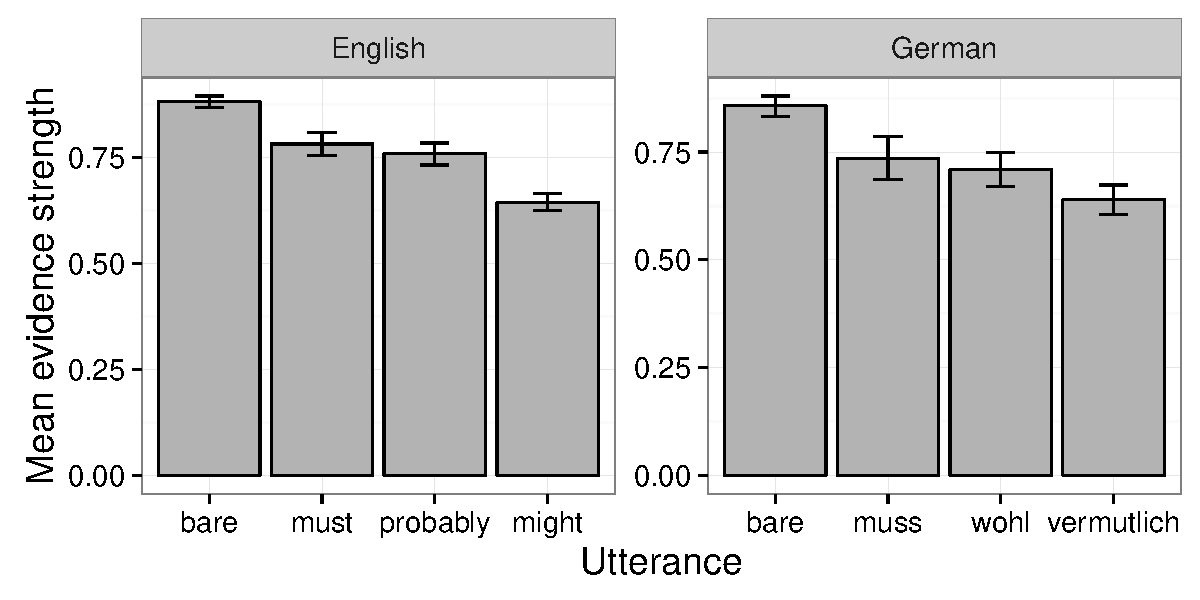
\includegraphics[width=.9\textwidth]{pics/mean-production-evidence}\caption{Mean strength of evidence given when using each utterance, for English (left) and German (right). Error bars indicate bootstrapped 95\% confidence intervals.}
\label{fig:utterances-estrength}
\end{figure}

\begin{figure}
\centering
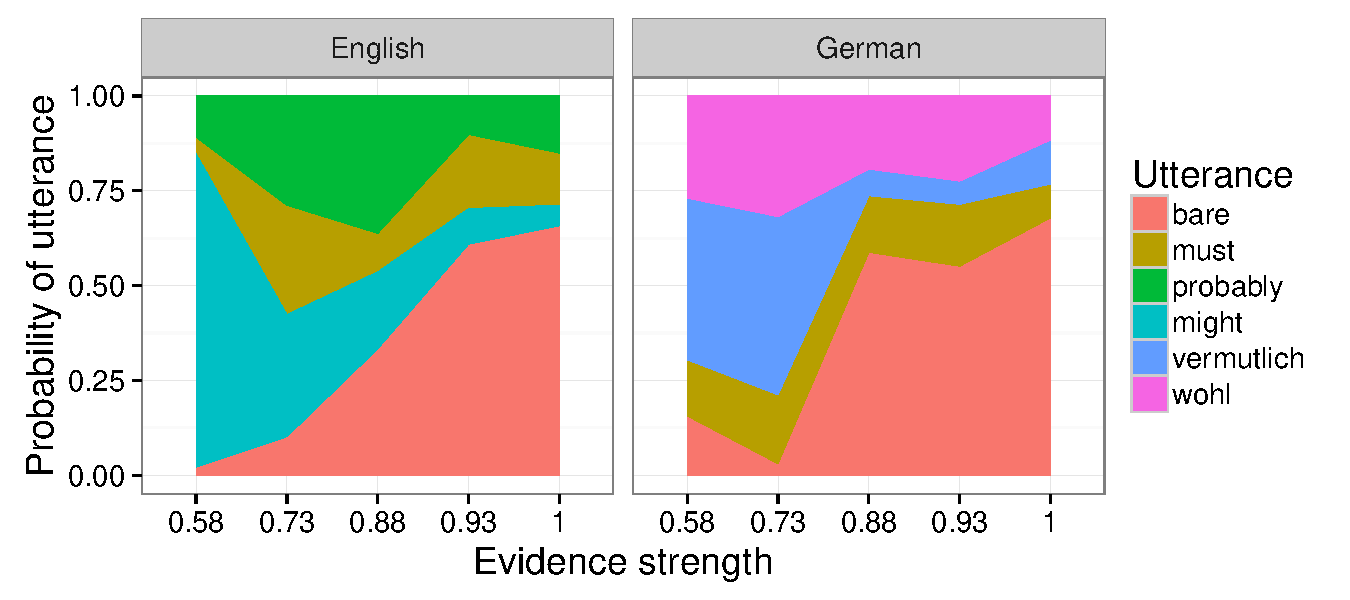
\includegraphics[width=\textwidth]{pics/production-by-strength}\caption{Probability of utterance choice as a function of evidence strength for English (left) and German (right). X-axis labels indicate the maximum evidence strength for the bin that the utterance proportion was computed over.}
\label{fig:utterances-by-strength}
\end{figure}

\subsection{Discussion}
We interpret these results as follows. First, bare utterances result from maximally-strong evidence: when certainty of \emph{p} is high, the claim that \emph{p} may be made directly. As evidence strength decreases, speakers employ evidential devices that track evidence strength. In German, due to the lexical inventory of discourse particles, speakers have a choice of using epistemic adverbs such as \emph{vermutlich}, epistemic \emph{muss}, and particles like \emph{wohl}. As \figref{fig:utterances-estrength} shows, speakers tend to use \emph{muss} and \emph{wohl} instead of the respective adverb when the degree of evidence strength is higher. In other words, when investigating the dependence on evidence strength for \emph{p}, we find that \emph{muss} and \emph{wohl} pattern together, in contrast to other modal means such as \emph{vermutlich}. This is in line with the ideas put forward by \cite{Zimmermann2004, Zimmermann2008}: discourse particles, in contrast to modal adverbs, do not add epistemic uncertainty to the presupposition of an utterance. That is, the particle leaves the asserted state of affairs untouched, and thus we could expect the speaker to be more committed to the truth of the proposition when using a particle than when using a synonymous adverb expressing weakened commitment. Given our results, it might be that epistemic \emph{must}/\emph{muss} also does not add the effect of weakened commitment to the presupposition of an utterance, as our sketch in Section 1 already indicated. Rather, weakened speaker commitment in this case is derived by separate (and additional) interpretive mechanisms that account for the failed inference involved in interpreting epistemic \emph{must} (see Section 1). This could explain the difference we observe when comparing \emph{must} with other modal means (such as \emph{might} and \emph{probably}) that operate within the truth-conditional content of an utterance. We will come back to this issue in more detail below.



\section{Experiment 3a: comprehension (listener belief)}


We next tested the flip side of the communicative coin: What are the inferences that listeners draw upon observing the various evidential devices explored in Exp.~2? In particular, depending on the utterance $u$ used to communicate about $p$, (i) how strong are listeners' resulting beliefs in $p$; (ii) what do they take the speaker to be committed to in uttering $u$; and (iii)  what do they believe to be the strength of the evidence for $p$ the speaker was in possession of when producing $u$? Exp.~3a addresses questions (i) and (iii) and Exp.~3b addresses questions (ii) and (iii). We first report Exp.~3a.\footnote{The English version of this experiment can be viewed \href{http://stanford.edu/~jdegen/72_modals_comprehension_evidence_room/modals.html}{here} and the German version \href{http://web.stanford.edu/~jdegen/cgi-bin/2_dp_comprehension_listenerbelief/modals.html}{here}.} The English and German experiments were identical except for the language of testing and the target utterances presented to participants: English participants saw the set in \eref{utterancechoices},  German participants the one in \eref{gutterancechoices}.

\subsection{Methods}

\subsubsection{Participants}

For the English version, we recruited 60 participants through Amazon's Mechanical Turk. 
For the German version, we recruited 60 participants through the German crowd-sourcing service Clickworker. Participants were compensated for their participation.

\subsubsection{Materials and procedure}

Participants were presented with an utterance \emph{u} (e.g., ``It must be raining'') and asked to both rate the probability of the state of affairs \emph{p} obtaining (e.g., it is raining) and to select one out of five pieces of evidence that the speaker most likely had about \emph{p} in choosing the utterance. On each trial, participants first saw two context sentences: ``You are in a windowless room. Your friend X walks in and says: […],’’ where ``X'' was a randomly generated name.\footnote{This was done to discourage effects of inferences about speaker-specific language use on interpretation.} Participants then saw one of the utterances from Exp.~2 that ``X'' produced, e.g., ``It must be raining.’’ They were then asked about the strength of their belief in $p$: ``How likely do you think it is that it is raining?'' and adjusted a slider with endpoints labeled ``impossible'' (coded as 0) and ``certain'' (coded as 1) in response. Once they indicated their belief in $p$, the five potential pieces of evidence previously used in Exps.~1 and 2 were shown and participants were asked to choose the one the speaker likely had: ``How do you think X knows about the rain?'' 

Participants provided one set of judgments for each domain, resulting in four trials per participant. Each participant saw each type of utterance (English: \emph{bare}, \emph{must}, \emph{probably}, \emph{might}; German: \emph{bare}, \emph{muss}, \emph{wohl}, \emph{vermutlich}) across trials. Utterance types were randomly distributed across domains. Trial order was randomized, as was the order in which pieces of evidence were displayed.

%In the German version, the procedure was identical, but materials were presented in German and the utterances participants observed were the ones used in the German version of Exp.~2.

\subsection{Results and discussion}

Two questions are of interest: first, does the probability of listener belief in $p$ vary as a function of the observed utterance? In other words, how are listeners' beliefs influenced by various evidential devices? Second, does the strength of the evidence for $p$ inferred to be available to the speaker vary as a function of the observed utterance? To address the first question, we conducted a mixed effects linear regression predicting degree of belief in $p$ from a dummy-coded utterance predictor with \emph{must}/\emph{muss} as reference level, separately for English and German. The model included random by-participant and by-item intercepts. Fig.~\ref{fig:expt3} shows mean probability of listener belief in $p$ by utterance: participants believed \emph{p} was more likely after observing the bare utterance than after observing the \emph{must} utterance in English  ($\beta$=.24, \emph{SE}=0.03, \emph{t}=9.1, \emph{p}$<$0.0001) and the \emph{muss} utterance in German ($\beta$=.22, \emph{SE}=0.03, \emph{t}=7.5, \emph{p}$<$0.0001). In contrast, in English they believed $p$ was less likely after observing \emph{might p} ($\beta$=-.09, \emph{SE}=0.03, \emph{t}=-3.44, \emph{p}$<$0.0008). There was no difference in resulting listener belief between \emph{must p} and \emph{probably p} ($\beta$=-.04, \emph{SE}=0.03, \emph{t}=-1.6, \emph{p}$<$0.12). And in German, there were no differences in degree of belief in $p$ between \emph{muss p} and \emph{vermutlich p} ($\beta$=-.02, \emph{SE}=0.03, \emph{t}=-.76, \emph{p}$<$.46) nor between \emph{muss p} and \emph{wohl p} ($\beta$=.01, \emph{SE}=0.03, \emph{t}=.43, \emph{p}$<$.67). %These results mirror the evidence strength effects found in production (Exp.~2), where we observed that speakers tend to use epistemic \emph{must}, \emph{muss} instead of corresponding modals when the degree of evidence strength is higher.

\begin{figure}
	\centering
	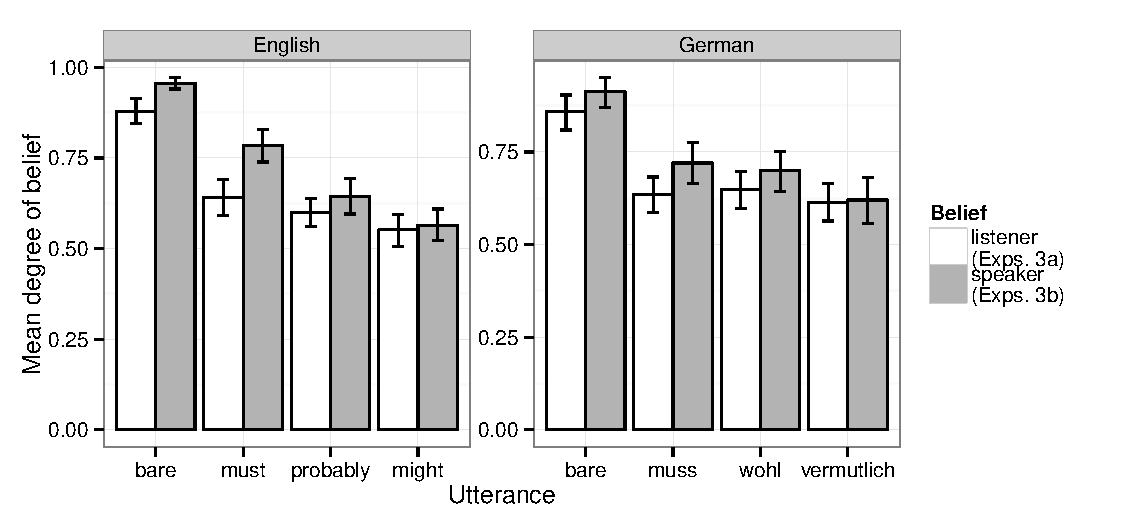
\includegraphics[width=\textwidth]{pics/mean-beliefs}
	\caption{Mean probability of listener and speaker belief in $p$ by utterance for English (left) and German (right). Error bars indicate 95\% bootstrapped confidence intervals.}
	\label{fig:expt3}
\end{figure}

To address whether inferred speaker evidence strength mirrors the production results in Section 3, we conducted another mixed effects linear regression, this time predicting inferred strength of evidence for $p$ from a dummy-coded utterance predictor with \emph{must}/\emph{muss} as reference level, separately for English and German. The model included random by-participant and by-item intercepts.  \figref{fig:exp3-evidence} shows mean evidence strength ascribed to speakers by utterance. Interestingly, in English, participants inferred stronger evidence was available to the speaker after observing the bare utterance than \emph{must p} ($\beta$=.08, \emph{SE}=.02, \emph{t}=3.74, \emph{p}$<$ .0003), but inferred evidence strength was no different for \emph{probably p} ($\beta$=.01, \emph{SE}=0.02, \emph{t}=.55, \emph{p}$<$ .59) or \emph{might p} ($\beta$=-.02, \emph{SE}=0.02, \emph{t}=-.89, \emph{p}$<$ .38). In German, participants inferred stronger evidence was available to the speaker after observing the bare utterance than \emph{muss p} ($\beta$=.08, \emph{SE}=.02, \emph{t}=3.23, \emph{p}$<$ .002). In addition, they inferred that the available evidence must have been weaker upon observing \emph{vermutlich p} ($\beta$=-.05, \emph{SE}=.02, \emph{t}=-2.1, \emph{p}$<$ .04), but inferred evidence strength was no different for \emph{wohl p} ($\beta$=.001, \emph{SE}=0.02, \emph{t}=.07, \emph{p}$<$ .95). %This shows again that \emph{wohl} patterns with epistemic \emph{muss}, as we already observed in the context of production in Section 3.

Taken together, the results of the current experiment on comprehension mirror those from production: bare utterances lead to the greatest degree of belief in $p$ while indicating that the speaker had access to maximally-strong evidence. Speaker belief and inferred evidence strength decrease with the epistemic modals; \emph{must}/\emph{muss} patterns with \emph{probably}/\emph{vermutlich}. Crucially, \emph{muss} also patterns with the discourse particle \emph{wohl}, whose evidential contribution most likely occurs in a dimension of meaning outside the core, compositional semantics. We observed the same similarity in behavior between \emph{muss} and \emph{wohl} in the context of production in Exp.~2. In Section 6 below, we will discuss these parallel effects (in both comprehension and production) in more detail.



\begin{figure}
	\centering
	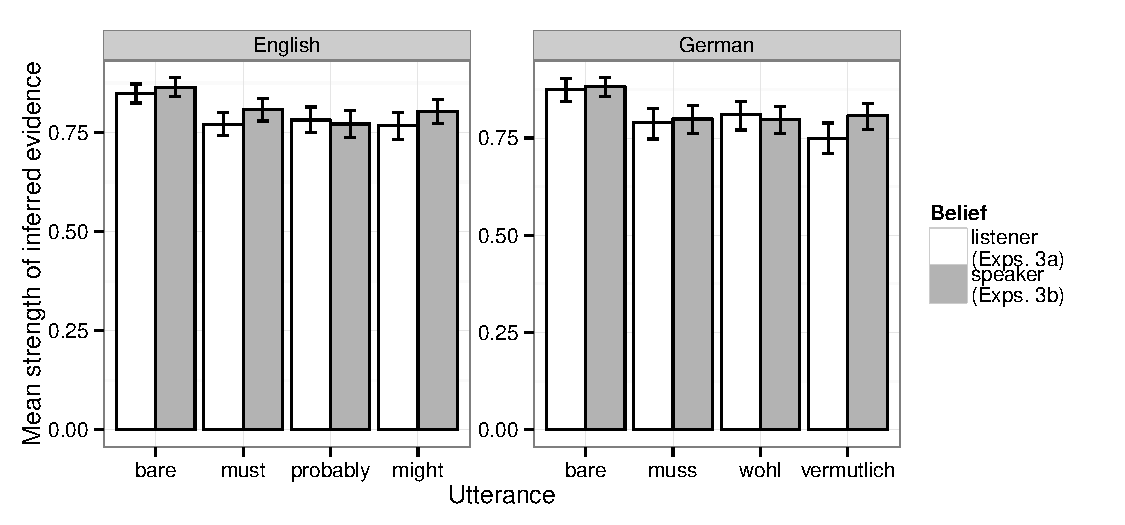
\includegraphics[width=\textwidth]{pics/mean-evidence}
	\caption{Mean inferred evidence strength by utterance for English (left) and German (right). Error bars indicate 95\% bootstrapped confidence intervals.}
	\label{fig:exp3-evidence}
\end{figure}

\section{Experiment 3b: comprehension (speaker commitment)}


Exp.~3a tested listener belief in $p$ as a function of the observed utterance. A related dimension is the commitment to the truth of $p$ that listeners ascribe to speakers. For example, a particular utterance may lead the listener to infer that the speaker is highly committed to (i.e., holds a strong belief in) $p$, while nevertheless not instilling the same degree of belief in $p$ in the listener. In fact, epistemic \emph{must} has been claimed to function like this: \cite{vonfintelgillies2010} claim that maximal speaker commitment is necessary for the use of epistemic \emph{must}, just as in the use of the bare form; yet in comprehension the interpretation of \emph{must p} is weaker than that of bare $p$. That is, after hearing \emph{must p}, listeners form beliefs in \emph{p} that are weaker than what they take to be speakers' beliefs in \emph{p}.  Exp.~3b thus tested the degree of belief in $p$ that listeners ascribe to \emph{speakers} depending on the utterance the speaker produced.\footnote{This experiment can be viewed \href{http://stanford.edu/~jdegen/80_modals_comprehension_speakerbelief/modals.html}{here}. The German version can be viewed \href{http://web.stanford.edu/~jdegen/cgi-bin/1_dp_comprehension_speakerbelief/discourse_particles.html}{here}.}

\subsection{Methods}

\subsubsection{Participants}

We recruited 60 English native speakers through Amazon's Mechanical Turk, and 60 German native speakers through Clickworker. Participants were compensated for their participation.

\subsubsection{Materials and procedure}

The design, procedure, and materials were identical to those of Exp.~3a with the exception of the dependent measure: instead of asking participants about their own strength of beliefs in $p$, they instead evaluated the speaker's belief in \emph{p}: ``Does X think that it's raining?'' Participants indicated their response by adjusting a slider on a scale with endpoints labeled ``Definitely not'' (coded as 0) and ``Definitely'' (coded as 1). 

\subsection{Results and discussion}

As in Exp.~3a, two questions are of interest: first, does the probability of  belief in $p$ -- this time, as ascribed to the speaker rather than the listener's own belief --  vary as a function of the observed utterance? Second, does the strength of the evidence for $p$ inferred to be available to the speaker vary as a function of the observed utterance? To address the first question, we conducted a mixed effects linear regression predicting degree of belief in $p$ from a dummy-coded utterance predictor with \emph{must}/\emph{muss} as reference level, separately for English and German. The model included random by-participant and by-item intercepts. Fig.~\ref{fig:expt3} shows mean probability of ascribed speaker belief in $p$ by utterance: participants believed the speaker was more likely to believe \emph{p}  after observing the bare utterance than after observing the \emph{must} utterance in English   ($\beta$=.18, \emph{SE}=0.03, \emph{t}=6.59, \emph{p}$<$0.0001) and the corresponding \emph{muss} utterance in German ($\beta$=.19, \emph{SE}=0.03, \emph{t}=5.79, \emph{p}$<$ .0001). In contrast, they believed the speaker was less likely to believe $p$ if they produced \emph{probably p} ($\beta$=-.14, \emph{SE}=0.03, \emph{t}=-5.28, \emph{p}$<$0.0001) or \emph{might p} ($\beta$=-.22, \emph{SE}=0.03, \emph{t}=-8.36, \emph{p}$<$0.0001). In German, participants believed the speaker was less likely to believe $p$ if they produced \emph{vermutlich p} ($\beta$=-.1, \emph{SE}=0.03, \emph{t}=-3.01, \emph{p}$<$0.004). There was no difference between \emph{muss p} and \emph{wohl p} ($\beta$=-.02, \emph{SE}=0.03, \emph{t}=-.61, \emph{p}$<$ .55).  This shows, similar to what we found in the domain of production, that speaker commitment in the case of both epistemic \emph{must} and discourse particles is stronger than in the case of using otherwise synonymous adverbs such as \emph{vermutlich}.

These results mirror the effects found in Exp.~3a, with the exception that all utterances led to differences in ascribed speaker commitment. Interestingly, the strength of the belief that participants attributed to speakers was stronger than their own resulting belief. This was borne out statistically in a model that was applied to both the listener and speaker belief datasets. This model was identical to that just reported, but additionally allowed for a dummy-coded belief holder predictor (listener vs.~speaker)  to interact with utterance. There was a clear main effect of belief holder, such that the belief ascribed to speakers was stronger than that held by listener participants, both in English ($\beta$=.14, \emph{SE}=0.03, \emph{t}=4.7, \emph{p}$<$0.0001) and in German ($\beta$=.08, \emph{SE}=0.04, \emph{t}=2.23, \emph{p}$<$ .03). Note that this suggests that \emph{must} is not special in generating the effect of stronger speaker commitment than resulting listener belief.

As in Exp.~3a, to address whether inferred speaker evidence strength mirrors production, we conducted another mixed effects linear regression, predicting inferred strength of evidence for $p$ from a dummy-coded utterance predictor with \emph{must}/\emph{muss} as reference level. The model included random by-participant and by-item intercepts.  \figref{fig:exp3-evidence} shows mean evidence strength ascribed to speakers by utterance:  again, participants inferred stronger evidence was available to the speaker after observing the bare utterance than \emph{must/muss q} in both English ($\beta$=.06, \emph{SE}=.02, \emph{t}=3.2, \emph{p}$<$ .002) and German ($\beta$=.08, \emph{SE}=.02, \emph{t}=4.05, \emph{p}$<$ .0001). However, inferred evidence strength was no different in English for \emph{probably p} ($\beta$=-.02, \emph{SE}=0.02, \emph{t}=-1.11, \emph{p}$<$ .27) or \emph{might p} ($\beta$=-.01, \emph{SE}=0.02, \emph{t}=-.49, \emph{p}$<$ .63); nor in German for \emph{vermutlich p} ($\beta$=-.0003, \emph{SE}=.02, \emph{t}=-.02, \emph{p}$<$ .99) or \emph{wohl p} ($\beta$=.008, \emph{SE}=0.02, \emph{t}=.36, \emph{p}$<$ .72).

Allowing this model to interact with a belief holder predictor and applying it simultaneously to the Exp.~3a dataset yields no main effect of belief holder in either English ($\beta$=.03, \emph{SE}=.02, \emph{t}=1.53, \emph{p}$<$ .13) or German ($\beta$=.0008, \emph{SE}=0.03, \emph{t}=.04, \emph{p}$<$ .97). This finding is unsurprising and serves as a sanity check for the belief holder effect, given that this aspect of the dependent measure was identical across experiments.


\section{General discussion and outlook}

In this squib, we presented a series of experiments focusing on the extent to which listeners' interpretation of certain types of modals and their judgments about speaker commitment differ in strength compared to the epistemic use of \emph{must}, to the use of discourse particles, and to statements with no modals at all. We demonstrated that speakers' production preferences for these different devices mirror the comprehension results under varying evidential circumstances.

Our results confirm some of the differences in strength of speaker commitment that different evidential devices have been claimed to give rise to. In particular, (i) the epistemic use of \emph{must}/\emph{muss} expresses a weaker commitment than the bare form and (ii) the use of the discourse particle \emph{wohl} conveys a stronger commitment than otherwise synonymous modal adverbs. However, in addition to experimentally confirming these well-established claims from the literature, we also illustrated interesting parallel effects of epistemic \emph{must}/\emph{muss} and the discourse particle \emph{wohl} — both in production and in comprehension. This finding might shed some new light on traditional assumptions: both epistemic  \emph{must}/\emph{muss} and discourse particles could involve a different interpretive route that listeners must take in order to arrive at the relevant reading of weakened speaker commitment. %In other words, the relative weakness of \emph{must}/\emph{muss} need not get encoded into its lexical semantics.

Consider the contribution of discourse particles: the listener interprets \emph{wohl} as belonging to the domain of ‘use-conditional content’ \citep{Recanati2004}, that is, to content that differs from ‘truth-conditional content’ (among other things) in being not challengeable. In terms of presuppositional semantics, the particle thus leaves the asserted state of affairs untouched, and thus we expect the speaker to be more committed to the truth of the proposition when using a particle than when using a synonymous adverb expressing weakened commitment. %As for the case of epistemic \emph{must}, our experiments lend support to the idea that \emph{must} crucially differs from other modal devices such as \emph{might} and \emph{probably}. 

The fact that \emph{muss} in German patterns with use-conditional expressions like discourse particles might suggest an account of epistemic \emph{must} that refrains from engineering the effect of weakness into the descriptive content of the utterance. Instead, we may assume that the notorious weakening effect is part of a non-propositional domain of utterance interpretation: The relatively weak interpretation of \emph{must}/\emph{muss} does not require encoding weakness or indirectness or evidential meaning into the semantics of modals. Under the assumption that the cost of uttering \emph{must p} is greater than the bare form (in simple terms, the \emph{must} utterance contains more words), listeners detect a M(arkedness)-implicature \citep{levinson2000}. 

This M-implicature proceeds as follows: \emph{must p} is marked (i.e., costly) relative to the bare form; the bare form is sufficiently strong already to convey \emph{p} (e.g., that it is raining), so listeners take the marked form to convey (i) the marked meaning that the speaker arrived at the conclusion \emph{p} via an evidentially less certain route than if they had chosen the shorter, bare form; and (ii) that the probability of \emph{p} is lower than it would have been had the utterance been the less costly bare $p$. Thus, the semantics of \emph{must} remains strong, as indicated in Section 1, and pragmatics does the job of weakening. In fact, already in \citet[pp.~33--34]{grice1989} do we find inspiration for this calculation that leads to the relative weakness of \emph{must}:

\begin{quotation}
``A wants to know whether \emph{p}, and B volunteers not only the information that \emph{p}, but information to the effect that it is certain that \emph{p}\ldots\ B's volubility may be undesigned, and if it is so regarded by A it may raise in A's mind a doubt as to whether B is as certain as he says he is\ldots\ But if it is thought of as designed, it would be an oblique way of conveying that it is to some degree controversial whether or not \emph{p}.''
\end{quotation}

%Rather than engineering weakness relative to bare \emph{p} directly into the meaning of the word \emph{must}, our account derives its weakness as an M-implicature 

All in all, given that the theoretical literature both on English modals and epistemic \emph{must} and on German discourse particles is based on subtle judgments of utterances, our paper for the first time presents an experimental investigation on cross-linguistic expressions conveying different strengths of speaker commitment. Our data thus contribute to a domain of research on speaker commitment that is only just taking shape at the crossroad of theoretical semantics/pragmatics and psycholinguistics, and we hope that we have provided a good starting point for approaching theoretical debates on the nature of evidential expressions empirically.





\section*{Author's addresses}
\begin{enumerate}
\item \emph{Judith Degen}\\ Department of Psychology\\ Stanford University\\ 450 Serra Mall\\ Stanford, CA 94305\\ jdegen@stanford.edu
\item \emph{Andreas Trotzke}\\ Stanford University\\ Center for the Study of Language and Information\\ 210 Panama St \\ Stanford, CA 94305\\ trotzke@stanford.edu
\item \emph{Gregory Scontras}\\ Department of Psychology\\ Stanford University\\ 450 Serra Mall\\ Stanford, CA 94305\\ scontras@stanford.edu
\item \emph{Eva Wittenberg}\\ Department of Linguistics \\ 9500 Gilman Drive\\
La Jolla, CA 92093-0108\\ ewittenberg@ucsd.edu
\item \emph{Noah D.~Goodman}\\ Department of Psychology\\ Stanford University\\ 450 Serra Mall\\ Stanford, CA 94305\\ ngoodman@stanford.edu
\end{enumerate}


\section*{Acknowledgments}
We would like to thank Justine Kao for support in designing the English series of experiments. This work was supported by ONR grant N00014-13-1-0788 and by a James S. McDonnell Foundation Scholar Award to NDG. AT gratefully acknowledges financial support from the German Research Foundation (DFG grants TR 1228/2-1 and BA 1178/9-1) and from the DFG Excellence Initiative (University of Konstanz, project no. 610/14). This research was further supported by an SNSF Early Postdoc. Mobility fellowship to JD and a postdoctoral fellowship to EW by the German Academic Exchange Service (DAAD).


%\bibliographystyle{apacite} % won't work for Greg
  \bibliographystyle{chicago} 

%\setlength{\bibleftmargin}{.125in}
%\setlength{\bibindent}{-\bibleftmargin}

\bibliography{bibs}
\appendix

\section{Pieces of evidence}
\label{sec:evidence}

This section lists, for each proposition $p$, the five pieces of evidence that were used throughout all experiments.

\subsection{It's raining. / Es hat geregnet.}

\begin{enumerate}
	\item You look out the window and see raindrops falling from the sky. \\ Sie sehen aus dem Fenster und beobachten, wie Regentropfen vom Himmel fallen. 
	\item You hear the sound of water dripping on the roof. \\ Sie können hören, wie Wasser auf das Dach prasselt.
	\item You check the weather report on the Internet, which says it is raining. \\ Sie haben im Internet den Wetterbericht gelesen, in dem stand, dass es regnen würde. 
	\item You see a person come in from outside with wet hair and wet clothes. \\ Sie sehen, wie jemand mit nassen Haaren und durchnässten Kleidern von draußen hereinkommt.
	\item Earlier today, you had seen dark clouds in the sky. \\ Sie haben heute Vormittag dunkle Wolken am Himmel gesehen.
\end{enumerate}

\subsection{The coffee is cold. / Der Kaffee ist kalt geworden.}

\begin{enumerate} 
	\item You take a sip of the coffee and feel that it is cold. \\
	Sie trinken einen Schluck Kaffee und stellen fest, dass er kalt ist
	\item You touch the coffee cup and feel that it is cold.\\
	Sie berühren die Kaffeetasse und stellen fest, dass sie kalt ist.
	\item You see that there is no steam coming from the coffee.\\
	Sie sehen, dass aus dem Kaffee kein Dampf aufsteigt.
	\item You know that the coffee has been on the table for an hour.\\
	Sie wissen, dass der Kaffee seit einer Stunde auf dem Tisch steht.
	\item You see that the cup isn't insulated.\\
	Sie sehen, dass die Tasse nicht isoliert ist.
\end{enumerate}

\subsection{Dinner is ready. / Das Abendessen ist fertig geworden.}

\begin{enumerate}
	\item You just prepared dinner and set it out on the table.\\
	Sie haben gerade das Abendessen zubereitet und auf den Tisch gestellt
	\item Your spouse tells you that dinner is ready.\\
	Ihr/e Partner/in sagt, dass das Abendessen fertig ist.
	\item Dinner is usually ready at around 6pm. You look at the clock and it is 6pm.\\
	Sie wissen, dass das Abendessen normalerweise um 18 Uhr fertig ist. Ein Blick auf die Uhr zeigt, dass es gerade 18 Uhr ist.
	\item You smell food coming from the dining room.\\
	Sie vernehmen den Geruch von Essen, der aus dem Esszimmer kommt.
	\item You're hungry.\\
	Sie haben Hunger.
\end{enumerate}

\subsection{The neighbor's dog is barking. / Der Nachbarshund hat gebellt.}

\begin{enumerate}
	\item You look outside and see Fluffy, the neighbor's dog, standing on the porch and barking.\\
	Sie schauen aus dem Fenster und sehen Struppi, den Hund der Nachbarn, wie er am Zaun steht und bellt.
	\item You hear the sound of a dog barking.\\
	Sie hören einen Hund bellen.
	\item You are listening to music with your earphones. You know that your neighbor's dog often barks in the evening.\\
	Sie haben Kopfhörer auf und hören Musik, wissen aber, dass der Hund der Nachbarn abends oft bellt.
	\item You are listening to music with your earphones. You look out the window and see that the mailman has just arrived at your neighbor's doorstep, when all of a sudden he jumps back.\\
	Sie haben Kopfhörer auf und hören Musik, sehen aber aus dem Fenster und beobachten, wie der Postbote vor der Nachbarstür einen Satz nach hinten macht.
	\item Your neighbor just got a new dog.\\
	Sie wissen, dass sich die Nachbarn gerade einen Hund angeschafft haben.
\end{enumerate}

\end{document}
